The advanced usage of CUP in this chapter includes:
\begin{itemize}
    \item
    grammars with ambiguities;
    \item
    lists;
    \item
    operator precedence;
    \item
    handling syntax errors.
\end{itemize}

\section{Ambiguous Grammars in CUP}
Conflicts can arise when the grammar is ambiguous; this implies that the parser must choose between two or more alternative actions.
The problem can be resolved by modifying the grammar (in order to make it non-ambiguous) or by instructing the parser on how to handle ambiguity.
The latter option requires that the parsing algorithm is fully understood, in order to avoid unwanted/wrong behaviors.

A grammar is ambiguous if there is at least one sequence of symbols for which two or more distinct parse trees exist.

Example:
\begin{lstlisting}
S ::= M;
M ::= 'if' C M;
M ::= 'if' C M 'else' M;
M ::= ID '=' NUM ';'
    | ID '=' ID ';';
C ::= '(' VAR '==' NUM ';';
\end{lstlisting}
This grammar is ambiguous; it is possible to convert it to this way:
\begin{lstlisting}
S ::= M
    | U;
U ::= 'if' C S;
U ::= 'if' C M 'else' U;
M ::= 'if' C M 'else' M;
M ::= ID '=' NUM ';'
    | ID ';';
C ::= '(' ID '==' NUM ')';
\end{lstlisting}

\subsection{Non-Ambiguous Grammar Example: Algebraic Expressions}
The non-ambiguous grammar that describes an algebraic expression is the following:
\begin{lstlisting}
S ::= E
E ::= E '+' T
E ::= E '-' T
E ::= T
T ::= T '*' F
T ::= T '/' F
T ::= F
F ::= '(' E ')'
F ::= NUM
\end{lstlisting}
The symbols \code{T} and \code{F} are used to solve the ambiguity given by the priority of operators ``\code{+}'' and ``\code{-}''.

\subsection{Ambiguous Grammar in CUP}
\subsubsection{Example of Shift-Reduce Conflicts}
Rules:
\begin{enumerate}
    \item
    \code{S :: = 'if' E 'then' S}
    \item
    \code{S :: = 'if' E 'then' S 'else' S}
    \item
    \code{S :: = V}
\end{enumerate}
The input is the following:
\begin{lstlisting}[mathescape]
if E then if E then V $\bullet$ else V
\end{lstlisting}

Stack situation:
\begin{figure}[H]
    \centerline{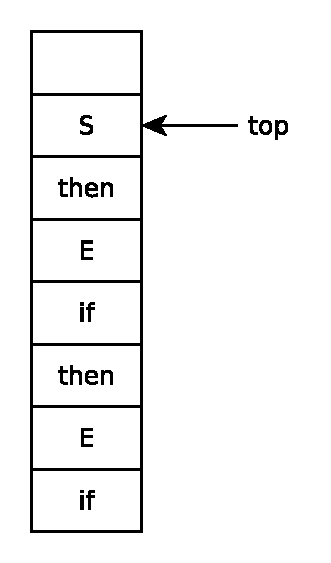
\includegraphics[width=0.2\textwidth]{img/20.pdf}}
\end{figure}

Possible actions:
\begin{enumerate}
    \item
    shift \code{else} token into the stack (rule 2);
    \begin{figure}[H]
        \centerline{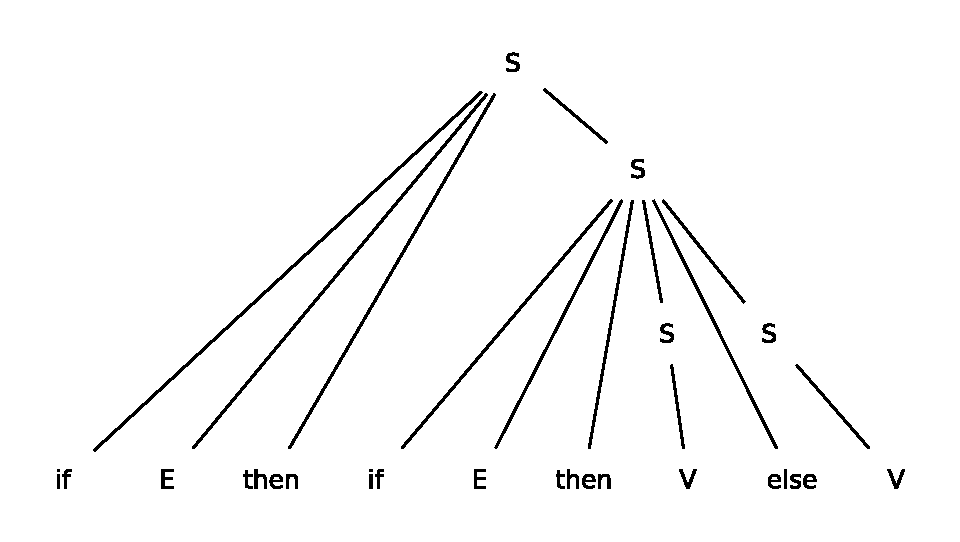
\includegraphics[width=0.6\textwidth]{img/21.pdf}}
    \end{figure}
    \item
    reduce the first four top elements of the stack (rule 1);
    \begin{figure}[H]
        \centerline{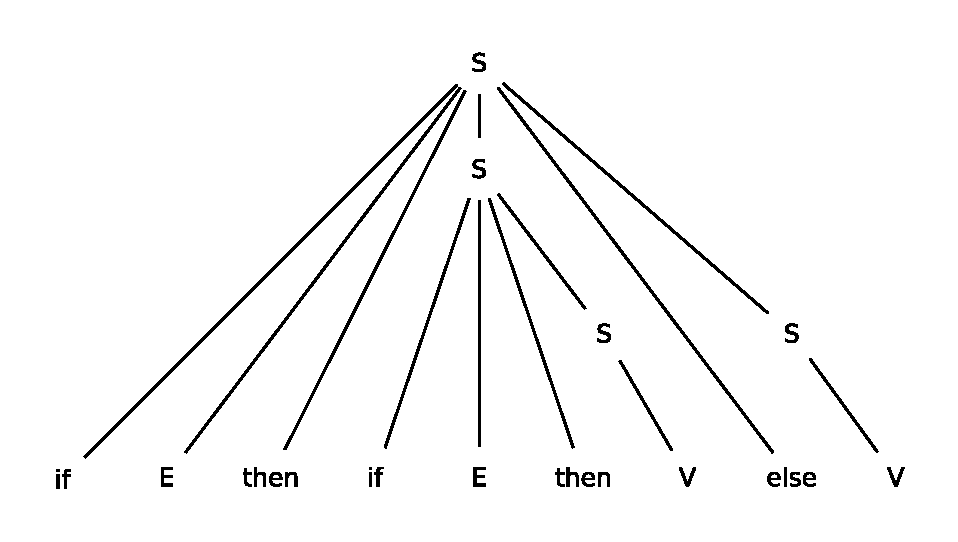
\includegraphics[width=0.6\textwidth]{img/22.pdf}}
    \end{figure}
\end{enumerate}

A possible solution is that CUP performs a Shift action and then the resulting parse tree is the following:
\begin{figure}[H]
    \centerline{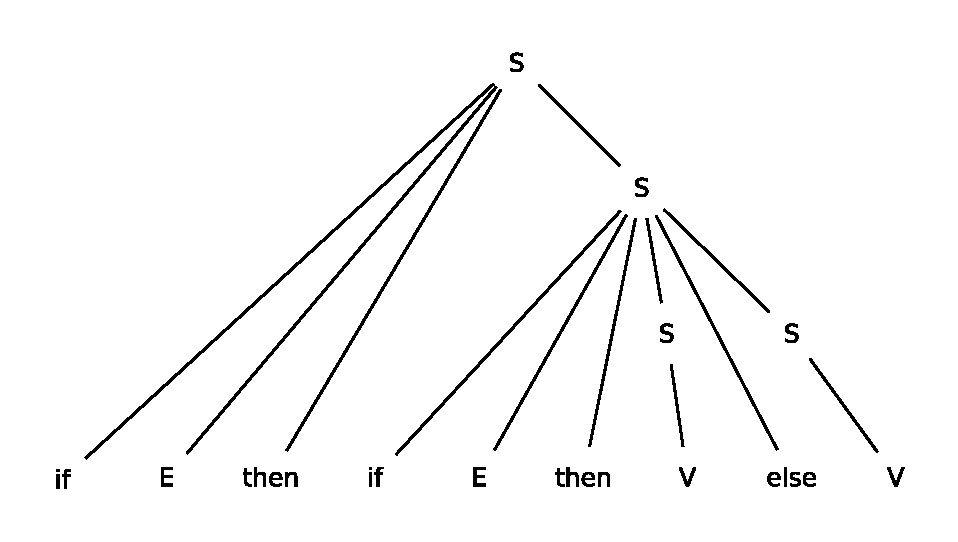
\includegraphics[width=0.6\textwidth]{img/23.pdf}}
\end{figure}

\subsubsection{Example of Reduce-Reduce Conflict}
Rules:
\begin{enumerate}
    \item
    \code{S :: = a B}
    \item
    \code{S :: = B}
    \item
    \code{S :: = a b}
    \item
    \code{S :: = b}
\end{enumerate}
The input is the following:
\begin{lstlisting}
a b
\end{lstlisting}
The next token is \code{EOF}.

Stack situation:
\begin{figure}[H]
    \centerline{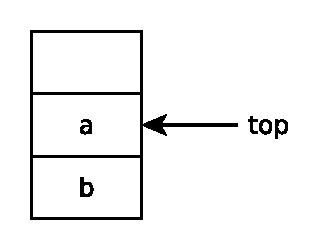
\includegraphics[width=0.2\textwidth]{img/24.pdf}}
\end{figure}
Two possible actions:
\begin{enumerate}
    \item
    reduce the first two top elements of the stack (rule 3);
    \begin{figure}[H]
        \centerline{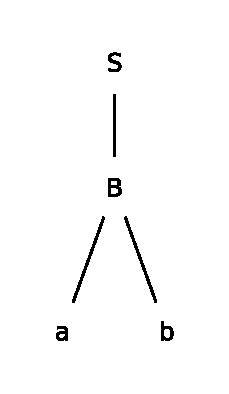
\includegraphics[width=0.17\textwidth]{img/25.pdf}}
    \end{figure}
    \item
    reduce the first top element of the stack (rule 4);
    \begin{figure}[H]
        \centerline{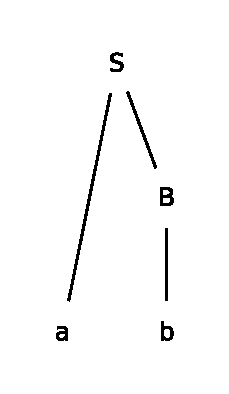
\includegraphics[width=0.17\textwidth]{img/26.pdf}}
    \end{figure}
\end{enumerate}
CUP can perform a reduction using the first defined rule (rule 3)\footnote{Simply because of rule order: rule 3 comes first than rule 4.}.

\section{Lists}
\subsubsection{Examples with Lists}
\begin{enumerate}
    \item
    List with at least one element \code{E}.
    \begin{lstlisting}
LIST ::= LIST E
    | E;
    \end{lstlisting}
    Parse tree:
    \begin{figure}[H]
        \centerline{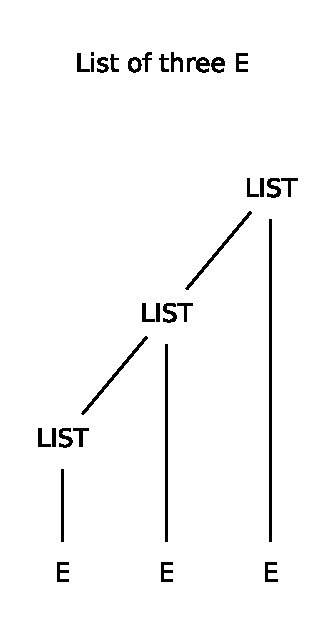
\includegraphics[width=0.25\textwidth]{img/27.pdf}}
    \end{figure}
    \item
    List of elements that can be empty.
    \begin{lstlisting}[mathescape]
LISTE ::= $\varepsilon$
    | LIST;
LIST ::= LIST E
    | $\varepsilon$;
    \end{lstlisting}
    Parse trees:
    \begin{figure}[H]
        \centerline{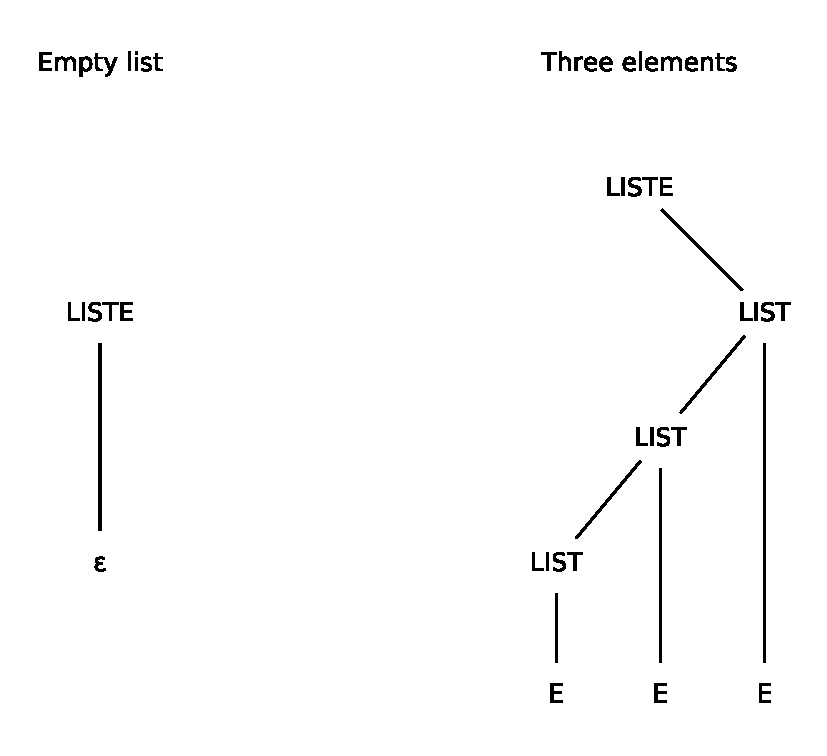
\includegraphics[width=0.6\textwidth]{img/28.pdf}}
    \end{figure}
    \item
    List of elements that can be empty.
    \begin{lstlisting}[mathescape]
LIST ::= LIST E
    | $\varepsilon$;
    \end{lstlisting}
    Parse trees:
    \begin{figure}[H]
        \centerline{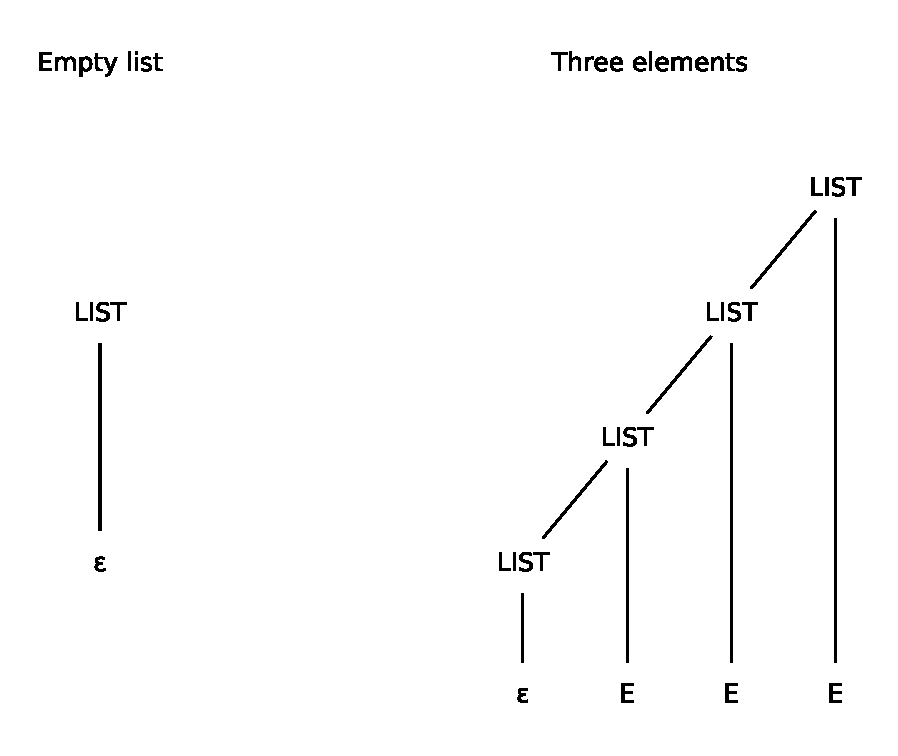
\includegraphics[width=0.6\textwidth]{img/29.pdf}}
    \end{figure}
    \item
    List of elements that can be empty (this example is actually incorrect).\footnote{It is ambiguous; see the two available ``three elements'' parse threes.}
    \begin{lstlisting}[mathescape]
LIST ::= LIST E
    | E
    | $\varepsilon$;
    \end{lstlisting}
    Parse trees:
    \begin{figure}[H]
        \centerline{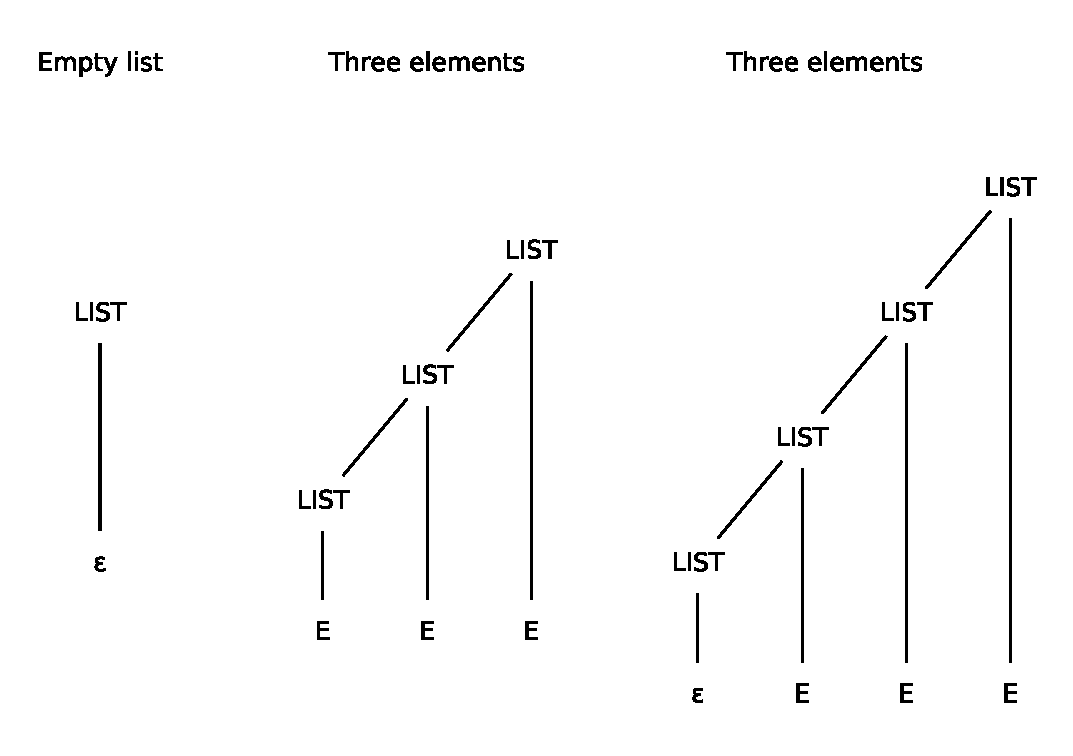
\includegraphics[width=0.8\textwidth]{img/30.pdf}}
    \end{figure}
    \item
    List of at least three elements.
    \begin{lstlisting}
LIST ::= LIST E
    | E E E;
    \end{lstlisting}
    Parse tree:
    \begin{figure}[H]
        \centerline{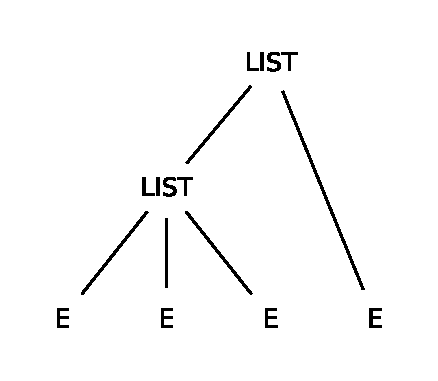
\includegraphics[width=0.35\textwidth]{img/31.pdf}}
    \end{figure}
    \item
    List of at least three elements in a odd number.
    \begin{lstlisting}
LIST ::= LIST E E
    | E E E;
    \end{lstlisting}
    Parse tree:
    \begin{figure}[H]
        \centerline{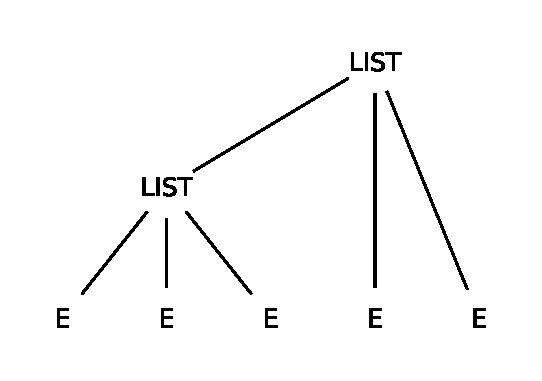
\includegraphics[width=0.4\textwidth]{img/32.pdf}}
    \end{figure}
\end{enumerate}

\section{Precedence Section: Ambiguous Grammars}
Ambiguous grammars can result in fewer, simpler rules, and hence can be sometimes preferred.
It is necessary to provide disambiguating rules in those cases.

% In the following example a walkaround has been used to center the example code.
Example:
\begin{center}
    Ambiguous grammar:
    \begin{lstlisting}
                                    E ::= E '+' E
                                    E ::= E '-' E
                                    E ::= E '*' E
                                    E ::= E '/' E
                                    E ::= '(' E ')'
                                    E ::= integer
    \end{lstlisting}
    $$
    \Downarrow
    $$
    Non-ambiguous grammar:
    \begin{lstlisting}
                                    S ::= E
                                    E ::= E '+' T
                                    E ::= E '-' T
                                    E ::= T
                                    T ::= T '*' F
                                    T ::= T '/' F
                                    T ::= F
                                    F ::= '(' E ')'
                                    F ::= integer
    \end{lstlisting}
\end{center}

\section{Associativity}
\subsubsection{Left-Associative Operator}
Example:
\code{E ::= E '+' E} $\Rightarrow 1 + 2 + 3 + 4 \to 3 + 3 + 4 \to 6 + 4 \to 10$

\subsubsection{Right-Associative Operator}
Example:
\code{E ::= E '+' E} $\Rightarrow 1 + 2 + 3 + 4 \to 1 + 1 + 7 \to 1 + 9 \to 10$

The assignment operator \code{'='} is right-associative: $a = b = 3$

The power operator is also right-associative: $3^{2^{2}} \to 3^4 \to 81$

\section{Precedence Section: Operators}
Example:
\begin{enumerate}
    \item
    \code{E ::= E '+' E}
    \item
    \code{E ::= E '*' E}
    \item
    \code{E ::= '(' E ')'}
    \item
    \code{E ::= int}
\end{enumerate}
Rule (1) (as well as rule (2)) is ambiguous because the associativity of the operator \code{'+'} (\code{'*'}) is not specified.
Moreover, the precedence of \code{'+'} and \code{'*'} is not specified by rules (1) and (2).
It is possible to make these rules non ambiguous by adding information in the precedence section.

The keyword ``precedence left'' defines a left-associative operator, ``precedence right'' a right-associative operator, whereas ``precedence non associative'' defines a non-associative operators.
The order in which precedence keywords are declared is inversely proportional to their priority.

\subsubsection{Precedence Section: Disambiguating Rules}
To each production that contains at least one terminal defined as operator, CUP associates the precedence and associativity of the rightmost operator.
If the rule is followed by the keyword ``\code{\%prec}'', the precedence and associativity are those of the specified operator.
In the case of a shift-reduce conflict, the action corresponding to the highest precedence production is executed.
If the precedence is the same, associativity is used: left-associativity results in a reduce action, right-associativity results in a shift action.

Example:
\begin{lstlisting}[frame=single]
terminal uminus;

precedence left '+', '-'; /* low priority */
precedence left '*', '/';
precedence left uminus; /* high priority */

start with E;

E ::= E '+' E
    | E '-' E
    | E '*' E
    | E '/' E
    | '-' E %prec uminus
    | '(' E ')'
    | integer
\end{lstlisting}

\section{User Code}
Directives are available to insert user code directly in the parser.
They are useful for:
\begin{itemize}
    \item
    personalizing the parser behavior;
    \item
    adding code directly in the class that implements the parser;
    \item
    using a scanner generator different from the default one.
\end{itemize}
They are initialized by ``\code{\{:}''\dots``\code{:\}}''.
This code is executed before calling any scanner method, hence before any terminal symbol is passed to the parser.
It is used to initialize variables or to initialize the scanner in case JFlex is not used.

When CUP generates the Java file that implements the parser, two classes are defined:
\begin{itemize}
    \item
    \code{public class Parser extends java_cup.runtime.LR_parser}, Parser is the Java class that implements the parser and inherits different methods from the \code{java_cup.runtime.LR_parser} class;
    \item
    \code{class CUP\$parser\%actions}, this is the class where declared grammar rules are translated into a Java program; here, also semantic actions (i.e., the Java code related to each rule) are reported.
\end{itemize}
The \code{java_cup.runtime.LR_parser} class is implemented in the file \code{java_cup/runtime/LR_parser.java}, in the CUP installation directory.

\subsubsection{Parser Code \code{\{:}\ldots\code{:\}}}
The code is included in the parser class.
It is used to include scanning methods within the parser but usually to override parser methods (e.g., to override methods for error handling).

\subsubsection{Action Code \code{\{:}\ldots\code{:\}}}
The code included in this directive is copied as is in the \code{CUP\$parser\$action} class.
The code is reached only in the semantic action associated with grammar rules.
It is used to define procedures and variables to be used in the actions associated to the grammar (e.g., the symbol table).

Example: errors - printing line and column

Symbol constructors:
\begin{lstlisting}
public Symbol(int sym_id)
public Symbol(int sym_id, int left, int right)
public Symbol(int sym_id, Object o)
public Symbol(int sym_id, Object o, int left, int right)
\end{lstlisting}
Scanner:
\begin{lstlisting}[frame=single]
import java_cup.runtime.*;

...

%%
%cup
%line
%column

%{
    private Symbol symbol(int type) {
        return new Symbol(type, yyline, yycolumn);
    }
    private Symbol symbol(int type, Object value) { // semantic analysis
        return new Symbol(type, yyline, yycolumn, value);
    }
%}

...

%%
[a-z]   {return symbol(sym.EL);}
','     {return symbol(sym.CM);}
\end{lstlisting}
Parser:
\begin{lstlisting}[frame=single]
import java_cup.runtime.*;

parser code {:
    public void report_error(String message, Object info) {
        StringBuffer m = new StringBuffer(message);
        if(info instanceof Symbol) {
            if((((Symbol)info).left != -1) && (((Symbol)info).right != -1)) {
                int line = (((Symbol)info).left) + 1;
                int column = (((Symbol)info).right) + 1;
                m.append("(linea: " + line + ", colonna: " + column + ")");
            }
        }
        System.err.println(m);
    }
:}
\end{lstlisting}

\section{Handling Syntax Errors}
Generally speaking, when a parser finds an error, it should not immediately terminate the execution.
A compiler usually tries to recover from the error, in order to analyze the rest of the input and signal the highest possible number of errors.
As default a CUP-generated parser when an error is detected:
\begin{itemize}
    \item
    signals by means of the method \code{public void syntax_error(Symbol cur_token)} defined in \code{java_cup.runtime.LR_parser} class a syntax error, writing ``\emph{Syntax error}'' in \code{stderr};
    \item
    if the error is not managed by the parser, the \code{public void unrecovered_syntax_error(Symbol cur_token)} method, also defined in \code{java_cup.runtime.LR_parser}; this function, after writing ``\emph{Couldn't repair and continue parse}'' in \code{stderr} (to notify) stops the execution of the parser.
\end{itemize}

Analyzing the two functions:
\begin{itemize}
    \item
    \code{public void syntax_error(Symbol cur_token)} calls the function \code{report_error} with the following parameters: ``\emph{Syntax Error}'', and \code{cur_token}, where - when the error occurs - \code{cur_token} is the currently lookahead symbol;
    \item
    \code{public void unrecovered_syntax_error(Symbol cur_token)} calls the function\code{report_fatal_error}, with the following parameters: ``\emph{Couldn't repair and continue parse}'', \code{cur_token}.
\end{itemize}
The \code{report_fatal_error} function calls with the same parameters \code{report_error} and it launches an exception that causes the end of the parser.

A suitable redefinition, in parser code \code{\{:}\ldots\code{:\}}, of the listed functions, allows to customize errors management.

\subsection{\code{error} Predefined Symbol}
The \code{error} predefined symbol signals an error condition.
It can be used within the grammar in order to enable the parser to continue execution when an error is encountered.

Example:
\begin{lstlisting}
ass ::= ID EQ E S
    | ID EQ error S;
\end{lstlisting}

\subsubsection{How does CUP handle the \code{error} symbol?}
When an error occurs, the parser will start emptying the stack until a state is found in which the \code{error} symbol is allowed.\footnote{In the previous example, incorrect \code{E} are removed from the stack until the terminal \code{EQ} is found on the top of the stack.}
The \code{error} token is acceptable, the parser resumes syntax analysis, otherwise the parser will continue to read and discard token, until an acceptable one is found.\footnote{In the previous example, the parser will read and discard all tokens until \code{S} is found.}

\subsubsection{General Rules}
A simple strategy for error handling is skipping the current statement:
\begin{lstlisting}
stmt ::= error ';'
\end{lstlisting}
Sometimes it can be useful to find a closing symbol corresponding to an opening symbol:
\begin{lstlisting}
expr ::= '(' expr ')'
    | '(' error ')'
\end{lstlisting}
Note that to limit the generation of spurious error messages, after an error occurs, error signaling is suspended until at least three consecutive tokens are shifted.

Example:
\begin{lstlisting}[frame=single]
file ::= funcs;

funcs ::=
    | funcs func;

func ::= ID '(' ')' compound;

compound ::= '{' stmts '}';

stmts ::=
    | stmts stmt;

stmt ::= exp ';'
    | compound;

exp ::= NUM
    | exp '+' exp
    | exp '-' exp
    | exp '*' exp
    | exp '/' exp
    | '-' exp %prec neg
    | '(' exp ')';

stmt ::= exp ';'
    | compound
    | error ';' {: System.err.println("Syntax error"); :};

compound ::= '{' stmts '}'
    | '{' stmts error '}' {: System.err.println("Missing ';' before '}'"); :};

exp ::= '(' error ')' {: System.err.println("Syntax error in expression"); :};
\end{lstlisting}

\section{Attributes of Symbols}
A set of attributes can be associated to each symbol; attributes can be:
\begin{description}
    \item[synthesized] calculated from the values of the attributes of the node's children in the parse tree;
    \item[inherited] calculated from the values of the parents/siblings in the parse tree.
\end{description}

\section{Synthesized Attributes}
A grammar whose attributes are all synthesized is denoted as an S-attribute grammar.

In this case, it is possible to calculate the values of all attributes using a bottom-up strategy, from the leaves to the root of the parse tree.

Example:
\begin{lstlisting}[mathescape]
    E $\to$ E1 '+' T $\Rightarrow$ E.value ::= E1.value + T.value
    E $\to$ T $\Rightarrow$ E.value ::= T.value
    T $\to$ number $\Rightarrow$ E.value ::= number.value
\end{lstlisting}